\documentclass[tikz,border=8pt]{standalone}
\usepackage{amsmath,amssymb}
\usetikzlibrary{arrows.meta,automata,positioning,quotes}
\begin{document}
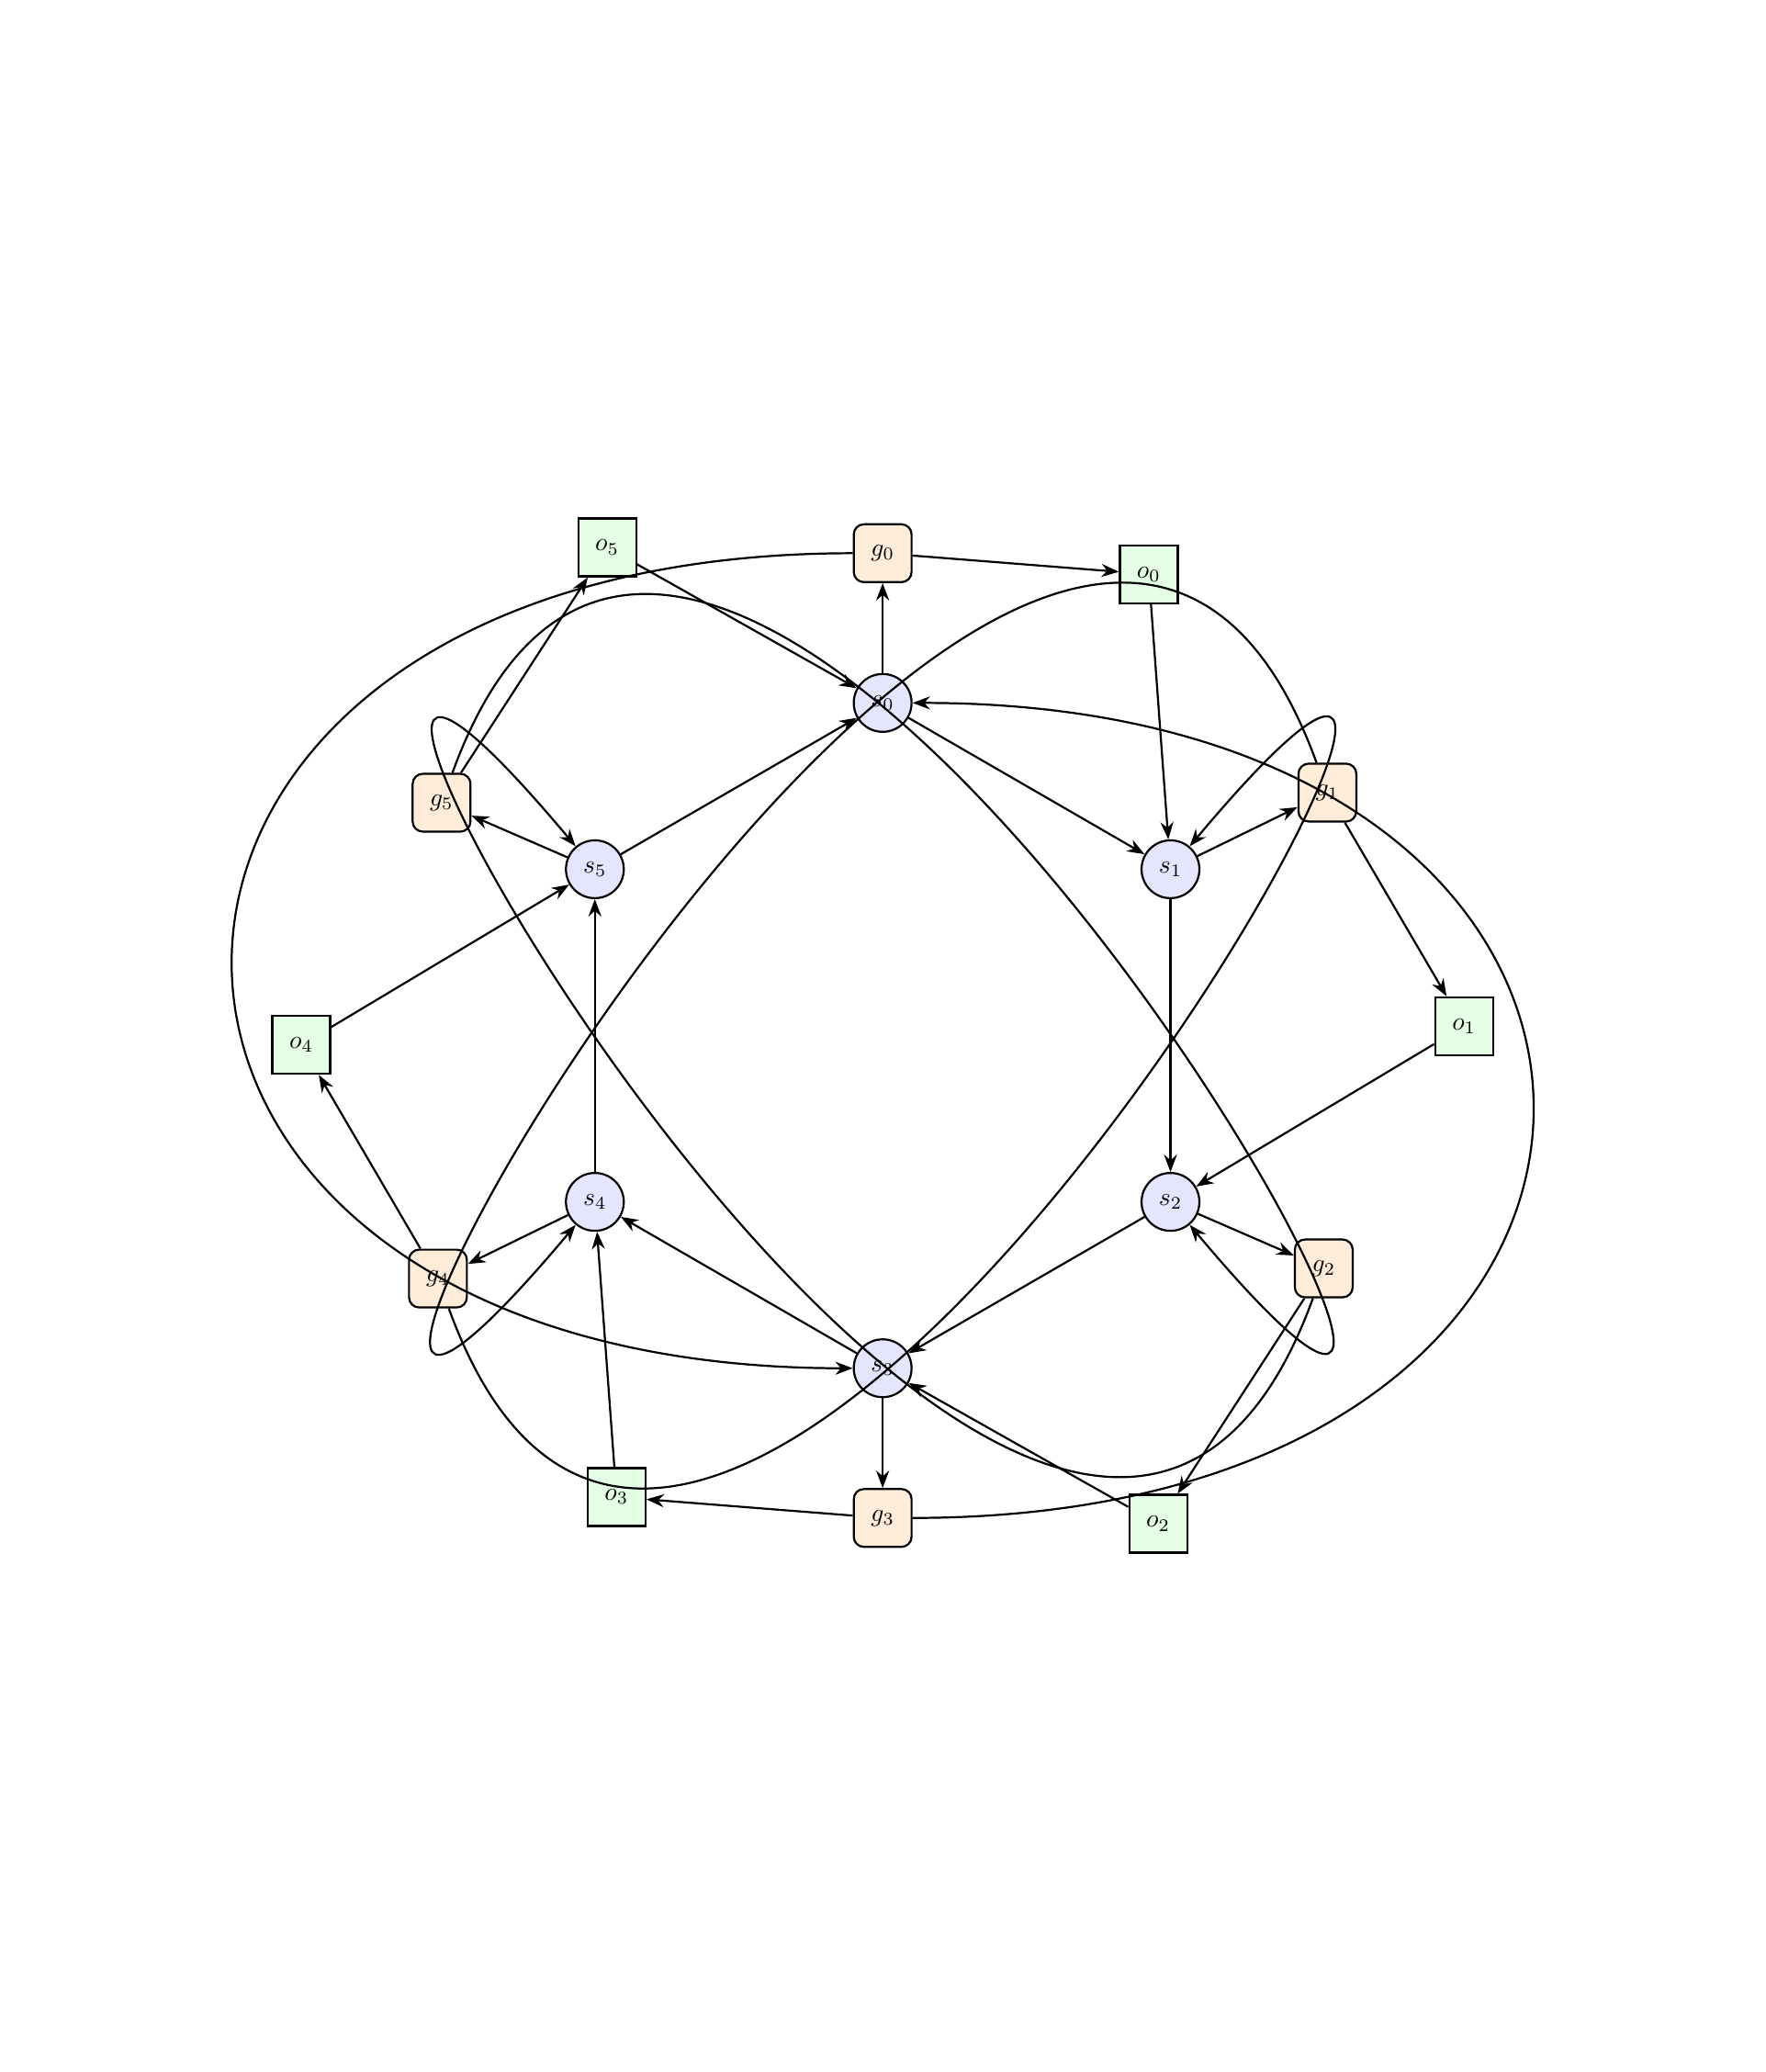
\begin{tikzpicture}[x=1cm,y=1cm]
\tikzset{
  graphnode/.style={circle,draw,thick,minimum size=8mm,inner sep=1pt,font=\sffamily},
  directed/.style={-{Stealth[length=2.4mm]},thick},
  undirected/.style={thick}
}
\node[graphnode,draw,circle,fill=blue!10] (n_s0) at (0.00,4.60) {$s_0$};
\node[graphnode,draw,circle,fill=blue!10] (n_s1) at (3.98,2.30) {$s_1$};
\node[graphnode,draw,circle,fill=blue!10] (n_s2) at (3.98,-2.30) {$s_2$};
\node[graphnode,draw,circle,fill=blue!10] (n_s3) at (0.00,-4.60) {$s_3$};
\node[graphnode,draw,circle,fill=blue!10] (n_s4) at (-3.98,-2.30) {$s_4$};
\node[graphnode,draw,circle,fill=blue!10] (n_s5) at (-3.98,2.30) {$s_5$};
\node[graphnode,draw,rectangle,rounded corners,fill=orange!15] (n_g0) at (0.00,6.67) {$g_0$};
\node[graphnode,draw,rectangle,rounded corners,fill=orange!15] (n_g1) at (6.15,3.36) {$g_1$};
\node[graphnode,draw,rectangle,rounded corners,fill=orange!15] (n_g2) at (6.10,-3.22) {$g_2$};
\node[graphnode,draw,rectangle,rounded corners,fill=orange!15] (n_g3) at (0.00,-6.67) {$g_3$};
\node[graphnode,draw,rectangle,rounded corners,fill=orange!15] (n_g4) at (-6.15,-3.36) {$g_4$};
\node[graphnode,draw,rectangle,rounded corners,fill=orange!15] (n_g5) at (-6.10,3.22) {$g_5$};
\node[graphnode,draw,rectangle,fill=green!10] (n_o0) at (3.68,6.38) {$o_0$};
\node[graphnode,draw,rectangle,fill=green!10] (n_o1) at (8.04,0.13) {$o_1$};
\node[graphnode,draw,rectangle,fill=green!10] (n_o2) at (3.81,-6.75) {$o_2$};
\node[graphnode,draw,rectangle,fill=green!10] (n_o3) at (-3.68,-6.38) {$o_3$};
\node[graphnode,draw,rectangle,fill=green!10] (n_o4) at (-8.04,-0.13) {$o_4$};
\node[graphnode,draw,rectangle,fill=green!10] (n_o5) at (-3.81,6.75) {$o_5$};
\draw[directed] (n_s0) -- (n_s1);
\draw[directed] (n_s1) -- (n_s2);
\draw[directed] (n_s2) -- (n_s3);
\draw[directed] (n_s3) -- (n_s4);
\draw[directed] (n_s4) -- (n_s5);
\draw[directed] (n_s5) -- (n_s0);
\draw[directed] (n_s0) -- (n_g0);
\draw[directed] (n_g0) -- (n_o0);
\draw[directed] (n_o0) -- (n_s1);
\draw[directed] (n_s1) -- (n_g1);
\draw[directed] (n_g1) -- (n_o1);
\draw[directed] (n_o1) -- (n_s2);
\draw[directed] (n_s2) -- (n_g2);
\draw[directed] (n_g2) -- (n_o2);
\draw[directed] (n_o2) -- (n_s3);
\draw[directed] (n_s3) -- (n_g3);
\draw[directed] (n_g3) -- (n_o3);
\draw[directed] (n_o3) -- (n_s4);
\draw[directed] (n_s4) -- (n_g4);
\draw[directed] (n_g4) -- (n_o4);
\draw[directed] (n_o4) -- (n_s5);
\draw[directed] (n_s5) -- (n_g5);
\draw[directed] (n_g5) -- (n_o5);
\draw[directed] (n_o5) -- (n_s0);
\draw[directed] (n_g0) to[out=180,in=180,looseness=2.6] (n_s3);
\draw[directed] (n_g1) to[out=110,in=230,looseness=2.3] (n_s4);
\draw[directed] (n_g2) to[out=250,in=130,looseness=2.3] (n_s5);
\draw[directed] (n_g3) to[out=0,in=0,looseness=2.6] (n_s0);
\draw[directed] (n_g4) to[out=290,in=50,looseness=2.3] (n_s1);
\draw[directed] (n_g5) to[out=70,in=310,looseness=2.3] (n_s2);
\end{tikzpicture}
\end{document}
